\chapter{The Pricing Problem}
\label{sec:the-pricing-problem}

\mytodo{These introductory paragraphs are either written like shit, duplicated or out-of-date. Please fix them.}

In this chapter we will cover in more details the pricing sub-problem
induced from the column generation scheme in BPC frameworks.
We've already the pricing problem in sections ....
In this chapter we will provide mathematical descriptions
of this problem by exploiting Integer Programming (IP).

\section{The Elementary Shortest Path Problem with Resource Constraints}
\label{sec:the-elementary-shortest-path-problem-with-resource-constraints}

\mytodo{These introductory paragraphs for the ESPPRC are either written like shit, duplicated or out-of-date. Please fix them.}

In this chapter we will introduce more formally the Elementary Shortest Path Problem with Resource Constraints (ESPPRC).
In this thesis we're interested in studying the ESPPRC induced from the PP when solving the RMP through a BPC framework employing the usage of robust inequalities only.

In the general case, the underlying network of ESPPRC problems may have negative cost cyles, which makes solving the ESPPRC an NP-hard problem \parencite{dror1994}.

As claimed in \textcite{dror1994}, the ESPPRC is an NP-hard problem,
However, the subproblem can be solved through a dynamic programming approach, as proposed by \textcite{feillet2004}.
The proposed algorithm is a natural extension of the Bellman–Ford algorithm \parencite{bellman1958, fordjr1956},
a common algorithm present in the "toolbelt" of all operations research practicioner,
which computes shortest paths from a source vertex to all other vertices,
by taking also in consideration additional path constraints.

While there may be multiple resources in play with different semantics
(time, capacity, gasoline, etc)
in the ESPPRC problem,
in this thesis we are mainly focused in ESPPRC subject to the single resource: the vehicle capacity.
Sometimes the ESPPRC subject to only the capacity constraint is called the Elementary Shortest
Path Problem with Capacity Constraints (ESPPCC).
It is however important to acknowledge that in the general case the ESPPRC allows for modeling
the pricing problems of many VRP variants such as the VRPTW, where also the "time resource"
plays a critical role.

Since we are not interested in non-robust cuts, the sub-problem
induced from the SP formulation coincides with an ESPPRC.
If non-robust cuts are employed, the sub-problem becomes
a slight variation of the EPSRRC which is characterized by additional constraints.

\medskip

In the case where the reduced cost network of the ESPPRC does not contain negative cost cycles
the elementarity condition does not need explicit modeling
and the resulting problem may be solved efficiently.
Some authors have proposed branch-and-bound
schemes applying the Lagrangian relaxation to the resource constraints
and by solving the associated shortest path
problem, through standard algorithms \parencite{beasley1989, carlyle2008}.

Other approaches for tackling the SPPRC use a
a tree-search scheme and a Lagrangian relaxation based
technique by employing standard unconstrained shortest path
algorithms, such as the Dijkstra algorithm \parencite{beasley1989}.

\medskip

\begin{comment}
\cite{bettinelli2010mathematical} ---------------
It is possible to address the pricing problem by optimizing its relaxation,
obtained by dropping the elementarity constraints. Solving a resource con-
strained shortest path problem (RCSPP) requires less computing time but
yields less tight lower bounds, since columns may include cycles. The two
different approaches have been followed for instance by Feillet et al. [42] and
Desrochers et al. [29] to solve the vehicle routing problem with time windows
(VRPTW) through column generation.
\end{comment}

\begin{comment}

[MY OWN STUFF, kept for reference purpose. TODO: Merge or delete later]
\subsection{Shortest Path Problem with Resource Constraints}
If there are no negative cost cyles, e.g. when the reduced cost variables are positive $\bar{c_{ij}} \ge 0$,
the ESPPRC problem is solvable in polynomial time, since the elementarity conditions are guaranteed
to be satisfied in this case.
In this particular case, some authors have proposed efficient methods to tackle this case:
\cite{beasley1989}, \cite{carlyle2008}, \cite{dumitrescu2003}, \cite{muhandiramge2009}.
These proposed approaches work under the assumption that no negative cost cycle is present,
and use lagrangian relaxation to relax the capacity constraints.

\subsection{Elementary Shortest Path Problem with Resource Constraints}
In the case where the network may be contain negative cost cycles, the
elementarity condition must be explicitly modeled, or relaxed, in order
to obtain reasonable dual bound solutions for the CVRP.
\textcite{feillet2004} proposes a dynamic programming algorithm where
the elementary property is handled through the usage of an additional resource
bound to each node.
\textcite{righini2006} proposes a bi-directional dynamic programming algorithm to solve the ESPPRC.
\end{comment}

\subsection{Integer Programming Model}
\label{sec:espprc-integer-programming-model}
The ESPPRC is traditionally defined over a \textbf{directed}
symmetric network.
The ESPRCC network is characterized by $N_0 + 2$ nodes,
where $N_0$ are the total number of customers for the original CVRP problem,
and the remaining two vertices represent the source and sink vertices used to
model a dissection of the depot node.
All the customers are edge-connected in both directions with one another,
while the source and sink vertex do not share direct connections.
The source and sink vertices are respectively forward connected and backward connected to all other customers.
where $V^\prime = V_0 \cup \Set*{0, N},\ |V^\prime| = N_0 + 2$.
The edges set $A^\prime$ can instead be expressed more formally as

\begin{equation}
	\begin{aligned}
		A^\prime = \  & \Set*{\Tuple*{i, j} \mid i, j \in V_0,\ i \ne j} \\
		              & \cup \Set*{\Tuple*{0, i} \mid i \in V_0}         \\
		              & \cup \Set*{\Tuple*{i, N} \mid i \in V_0}.
	\end{aligned}
\end{equation}

The edge set $A^\prime$ has size $|A^\prime| = N(N - 1) + 2(N - 1)$.
We formally define $\deltaplus(S) = \Set*{(i, j) \in A^\prime \mid i \in S, j \notin S}$
to denote the out-arcs crossing the set $S \subset V^\prime$.
Likewise, we define $\deltaminus(S) = \Set*{(i, j) \in A^\prime \mid i \notin S, j \in S}$
to denote the in-arcs crossing the set $S \subset V^\prime$.
For brevity’s sake,
we also define $\deltaplus(i) = \deltaplus(\Set*{i})$, $\deltaminus(i) = \deltaminus(\Set*{i})$
to denote respectively the singleton version of the in and out arcs for vertices $i \in V$.
Note that the conditions hold:
$\deltaplus(0) = V_0,\ \deltaminus(N) = V_0,\ \deltaminus(0) = \emptyset,\ \deltaplus(N) = \emptyset$.

At each directed edge $\Tuple*{i, j} \in A^\prime$ we have an associated weight $\bar{c_{ij}} \in \R$ which is directly linked to the dual variables of the RMP through the following equation:

\begin{equation}
	\bar{c_{ij}} = d_{ij} - \frac{\pi_i + \pi_j}{2} \quad \forall i, j \in V^\prime
\end{equation}

where $\pi$ represent the dual variables associated to constraints \eqref{eq:mp-customers-visited-by-exactly-one-route}\eqref{eq:mp-K-routes},
and to robust cutting-planes inequalities,
as was already explained in Section \ref{sec:column-generation-and-pricing-problem}.

Let $x_{ij} \in \Set*{0, 1} \quad \forall i, j \in V^\prime$ be a new set of binary variables
encoding feasible solutions for the ESPRCC problem (i.e. $x_{ij} = 1$ if edge $(i, j)$ is picked in the optimal path).
We can finally write the full ESPPRC IP formulation as:

\begin{align}
	\min_{x} \quad z_\mt{ESPPRC}(x) & =  \sum_{(i, j) \in A^\prime} \bar{c_{ij}} x_{ij} \label{eq:espprc-obj-function}                                                                                                               \\
	                                & \sum_{i \in V_0} \frac{q_i}{2} \Expr*{ \ExprESPPIngoingEdges{i} + \ExprESPPOutgoingEdges{i} }  \le Q                            \label{eq:espprc-resource-upper-bound-constraint}              \\
	                                & \ExprESPPIngoingEdges{i} = \ExprESPPOutgoingEdges{i}                                                \qquad \forall i \in V_0          \label{eq:espprc-flow-conservation-constraint-customers} \\
	                                & \ExprESPPOutgoingEdges[i]{0} = 1                                                                                                      \label{eq:espprc-flow-conservation-constraint-depot1}    \\
	                                & \ExprESPPIngoingEdges[i]{N} = 1                                                                                                       \label{eq:espprc-flow-conservation-constraint-depot2}    \\
	                                & \ExprESPPEdgesWithin[S] \le |S| - 1                                                                  \qquad \forall S \subseteq V^\prime,\ |S| \ge 2 \label{eq:espprc-sec-constraints}         \\
	                                & x_{0i} + x_{iN} \le 1                                                                                \qquad \forall i \in V_0         \label{eq:espprc-binding-directed}                       \\
	                                & x_{ij}                   \in \lbrace 0, 1 \rbrace                                                    \qquad \forall \Tuple*{i, j} \in A^\prime    \label{eq:espprc-x-mip-var-bounds}           \\
\end{align}

where, \eqref{eq:espprc-obj-function} is the objective function which we aim to minimize.
The remaining constraints characterize the set of feasible paths $P$, by paying attention that we are now dealing with
a directed network, and the depot node is duplicated twice.
Namely, constraint \eqref{eq:espprc-resource-upper-bound-constraint} expresses the resource bound modeled as a function of only the $x$ MIP variables,
constraint \eqref{eq:espprc-flow-conservation-constraint-customers} imposes a flow conservation for all vertices excluding the source and the sink node,
constraint \eqref{eq:espprc-flow-conservation-constraint-depot1}, \eqref{eq:espprc-flow-conservation-constraint-depot2} are the flow imposition for respectively the source and sink node,
constraint  \eqref{eq:espprc-binding-directed} avoids forming paths where a single customer is visited, this constraint is a direct consequence of the fact that the CVRP is defined over an undirected network,
constraint \eqref{eq:espprc-x-mip-var-bounds} imposes bound and integrality constraints on the $x$ MIP variables.

Finally, the most important inequalities, constraint \eqref{eq:espprc-sec-constraints}, represents the subtour elimination constraints.
These inequalities have two major impacts: first they avoid the form of spurious unconnected subtours, second they force the elementarity condition, namely they impose that each node must be visited at most once.
Two examples depicting respectively a solution containing spurious subtours and a non-elementary solution are provided in Figures \ref{fig:espprc-example-with-spurious-subtours} and \ref{fig:espprc-example-non-elementary-solution}.

\begin{figure}[ht]
	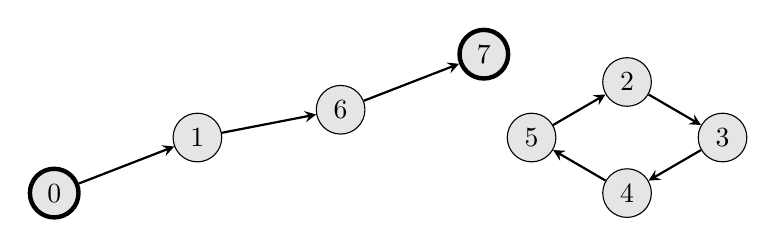
\begin{tikzpicture}[>=stealth, main/.style = {draw, circle, fill=black!10!white}]
		\centering

		\node[main, ultra thick] (0) at (0.1\textwidth,-20bp) {0};
		\node[main] (1) at (0.25\textwidth,0bp){1};
		\node[main] (6) at (0.4\textwidth,+10bp){6};
		\node[main, ultra thick] (7) at (0.55\textwidth,+30bp) {7};

		\node[main] (2) at (0.7\textwidth, +20bp){2};
		\node[main] (3) at (0.8\textwidth, -0bp) {3};
		\node[main] (4) at (0.7\textwidth, -20bp) {4};
		\node[main] (5) at (0.6\textwidth, -0bp) {5};

		\draw [->,thick] (0) -- (1);
		\draw [->,thick] (1) -- (6);
		\draw [->,thick] (6) -- (7);

		\draw [->,thick] (2) -- (3);
		\draw [->,thick] (3) -- (4);
		\draw [->,thick] (4) -- (5);
		\draw [->,thick] (5) -- (2);
	\end{tikzpicture}

	\centering
	\caption{An example of an ESPRRC solution containing spurious subtours.
		$V^\prime = \Set*{0, \dots, 7}$, ($0$ is the source vertex, $7$ the sink vertex).
		SEC inequalities, presented in \cref{eq:espprc-sec-constraints}, make the situation depicted in the figure impossible to occur.
	}
	\label{fig:espprc-example-with-spurious-subtours}
\end{figure}

\begin{figure}[ht]
	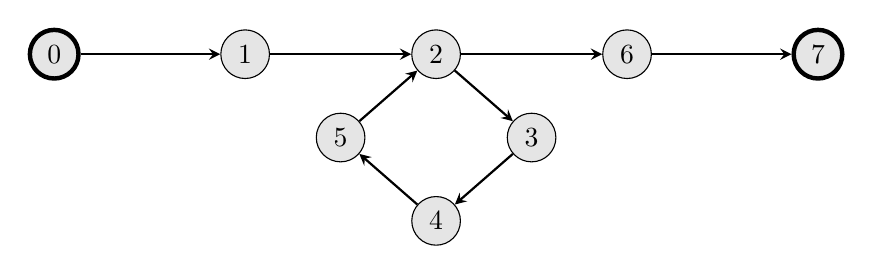
\begin{tikzpicture}[>=stealth, main/.style = {draw, circle, fill=black!10!white}]
		\centering

		\node[main, ultra thick] (0) at (0.1\textwidth,0bp) {0};
		\node[main] (1) at (0.3\textwidth,0bp){1};
		\node[main] (2) at (0.5\textwidth,0bp){2};
		\node[main] (3) at (0.6\textwidth,-30bp) {3};
		\node[main] (4) at (0.5\textwidth,-60bp) {4};
		\node[main] (5) at (0.4\textwidth,-30bp) {5};
		\node[main] (6) at (0.7\textwidth,0bp){6};
		\node[main, ultra thick] (7) at (0.9\textwidth,0bp) {7};

		\draw [->,thick] (0) -- (1);
		\draw [->,thick] (1) -- (2);
		\draw [->,thick] (2) -- (3);
		\draw [->,thick] (3) -- (4);
		\draw [->,thick] (4) -- (5);
		\draw [->,thick] (5) -- (2);
		\draw [->,thick] (2) -- (6);
		\draw [->,thick] (6) -- (7);
	\end{tikzpicture}

	\centering
	\caption{An example of an ESPRRC non-elementary solution.
		$V^\prime = \Set*{0, \dots, 7}$, ($0$ is the source vertex, $7$ the sink vertex).
		SEC inequalities, presented in \cref{eq:espprc-sec-constraints}, make the situation depicted in the figure impossible to occur.
	}
	\label{fig:espprc-example-non-elementary-solution}
\end{figure}

As done in \textcite{beasley1989} the elementarity condition can be relaxed by substituting constraint \eqref{eq:espprc-sec-constraints} in favour of:

\begin{equation}
	\sum_{i \in S} \sum_{j \in S}  x_{ij} \le M \sum_{i \in S} \sum_{j \in V^\prime \setminus S} x_{ij} \quad \forall S \subseteq V^\prime \setminus \Set*{N}
\end{equation}

where, $N = |V_0| + 1$ (recall $V_0$ is the set of customers) represents the sink vertex, and $M \in \R$ is a large positive constant.
In some cases, it is possible to relax the elementarity condition.
Relaxing the elementarity condition can simplify the pricing problem at the cost of obtaining weaker dual bounds for the RMP.

\section{The Capacitated Profitable Tour Problem}
\label{sec:the-capacitated-profitable-tour-problem}

The Capacitated Profitable Tour Problem, abbreviated as CPTP,
belongs to the group of the so-called travelling salesman
problems with profits (see \cite{feillet2005}),
and therefore presents many similarities with other very well known
problems such as:
(i) the Orienteering Problem (OP) \parencite{golden1987, laporte1990}
and (ii) the Profitable Tour Problem (PTP) \parencite{dellamico1995}.
The CPTP is an NP-hard combinatorial optimization problem representing
a distribution problem, in which,
given as input a set of customers
defined over a fully connected undirected network, the goal resides in finding
a resource constrained elementary tour (or circuit) starting from a common point called the depot,
that minimizes the overall travel distance while maximizing
the profits associated in serving only a subset of the customers.
The elementarity constraint dictates that no vertex
can be visited twice or more, thus implying that the earnable profit
per customer is available only once.
The CPTP can also be described in simple words
as a single-truck ($k = 1$) (C)VRP where it is possible to serve only a small set of customers,
based on a profit value that is gained when serving occurs.
The CPTP shows up naturally as a sub-problem in the column generation approach employed in solving many VRP variants.
It is an important special case of the ESPPRC, where the source and sink vertices coincide.
This problem is easier to describe than the ESPPRC,
however due to its narrower scope,
it is less addressed in the literature.
Instead, major contributions are dedicated in solving the ESPPRC through dynamic programming algorithms.

The few contributions studying the CPTP directly to solve the PP
are \cite{jepsen2011, jepsen2014}.

\subsection{Integer Programming Model}
\label{sec:cptp-integer-programming-model}

\textcite{letchford2013, jepsen2014} provided in their work an IP formulation for the CPTP.
The IP model presented in this section is derived from their work, and it is here summarized.

Let $G = \Tuple*{V, E}$ denote a complete undirected graph, where $V = \Set*{0, 1, \dots, N - 1}$ denotes the set of nodes,
$E = \Set*{e = (i, j) \mid i,j \in V, j \ge i + 1}$ the set of edges, and $N$ the number of nodes in the graph.
The value $0 \in V$ is used to denote the depot node.
For convenience, we define $V_0 = V \setminus \Set*{0}$ to express the set of customers, and $N_0 = N - 1$ to denote the number of customers.
Let $\delta(S)$ with $S \subseteq V$ denote the edges crossing the set $S$ and its complement $\overline{S} = V \setminus S$.
More formally we can express $\delta(S)$ as $\delta(S) = \Set*{ (i, j) \in E \mid i \in \Expr*{S \cap V}, j \in \Expr*{ \overline{S} \cap V } }$.
For brevity, we also define $\delta(i) = \delta(\Set*{i})$ to denote the set of edges incident to node $i \in V$.

Let $p_{i} \in \R, p_{i} \ge 0$ denote the profit function, and $q_{i} \in \R, q_{i} \ge 0$ denote the demand function, which represent respectively the profit gain and required demand in visiting a vertex $i \in V$.
By convention $q_0 = 0$, but notice that the profit at the depot is allowed to be $p_0 \ge 0$.
Let $d_{ij} \in \R, d_{ij} > 0$ denote the distance function between a pair of nodes  $i, j \in V$.
We assume that the distance function is symmetric $d_{ij} = d_{ji}$ and satisfies the triangle inequality $d_{ij} \le d_{ih} + d_{hj}$.

We define two sets of binary variables: $x_{ij}$, $y_{i} \in \Set*{0, 1}$, used to compose output solutions for the CPTP.
Together they model respectively an edge and a vertex as being part of the tour solution.

Given an upper bound $Q \in \R,Q \ge 0$ for the total resource consumption, we can finally express the CPTP problem as an integer programming formulation

\begin{align}
	\min_{x,y} \quad z_\mt{CPTP}(x, y) & =  \sum_{i \in V} \sum_{\EqStackTwo{j \in V}{j \ge i + 1}} d_{ij} x_{ij} - \sum_{i \in V} p_i y_i \label{eq:obj-function}                                                                                                                \\
	                                   & y_0 = 1                                                                                                                   & \label{eq:depot-part-of-tour-constraint}                                                                     \\
	                                   & \ExprCptpEdgesIncident{i}  = 2 y_i                                                                                        & \quad \forall i \in V         \label{eq:flow-conservation-constraint}                                        \\
	                                   & \ExprCptpFlowExiting{S} \ge 2 y_{i}                                                                                       & \quad \EqStackTwo{\forall i \in S}{\forall S \subseteq V_0,\ \SetSize*{S} \ge 2} \label{eq:gsec-constraints} \\
	                                   & \ExprCptpDemandSum  \le Q                                                                                                 & \label{eq:resource-upper-bound-constraint}                                                                   \\
	                                   & x_{ij}                   \in \Set*{0, 1}                                                                                  & \quad \forall (i, j) \in E               \label{eq:x-mip-var-bounds}                                         \\
	                                   & y_{i}                    \in \Set*{0, 1}                                                                                  & \quad \forall i \in V,\ i \ge 1          \label{eq:y-mip-var-bounds}
\end{align}

The equation \eqref{eq:obj-function} denotes the objective function, and it is made of two terms: the cost of traveling through the tour (positive contribution) and the total sum of the profits associated to visiting a subset of the vertices (negative contribution).
The constraint \eqref{eq:depot-part-of-tour-constraint} ensures that the depot is always visited.
Constraints \eqref{eq:flow-conservation-constraint} imposes flow conservation constraints for each vertex.
The equation \eqref{eq:gsec-constraints} are the generalized subtour elimination constraints \textbf{(GSECs)} and must be present to guarantee that the solution does not contain spurious unconnected subtours.
There is an exponential number of GSECs, as such, for performance reasons these constraints cannot be inserted statically in a MIP solver, and must instead be efficiently dynamically separated.
The equation \eqref{eq:resource-upper-bound-constraint} models the fact that a tour may visit any vertex as long as the total demand doesn't exceed the vehicle capacity.
Finally, the equations \eqref{eq:x-mip-var-bounds}, \eqref{eq:y-mip-var-bounds} specify the bounds and domain of the $x_{ij}$ and $y_{i}$ variables respectively.

The IP model consists of $\frac{N^2 + N}{2}$ number of binary variables.
If we ignore the GSECs and the binary variable bounds, the total number of constraints characterizing the model add up to $N + 2$.

Note that the IP formulation only permits solutions visiting at least three vertices (the depot and two customers).
We could allow for single customer solutions by relaxing the binary variable requirements and by modifying the IP model.
Instead, it may be simpler to take a different approach and leave the IP model as is.
By employing a bruteforce algorithm in $\Theta(N)$ time we can scan for improving single-customer solutions.
After the resolution of the IP model, we check for improving single-customer solutions and, if any exist, we update the incumbent.

\subsection{GSECs inequalities}\label{sec:gsec-inequality}

\mytodo{Add more details/history/literature about GSECs here.}

It may be interesting to study the relationship between the number of non-zero binary variables participating in a GSEC as a function of the set size $\SetSize*{S}$.
To achieve this we can express the size of the edge crossing set $\delta(S)$ as

\begin{equation}\label{eq:delta-s-set-size}
	\SetSize*{\delta(S)} = \SetSize*{S} (N - \SetSize*{S})
\end{equation}

which is maximized when $\SetSize*{S} = \frac{N}{2}$, thus leading to the following easy upper bound:

\begin{equation}\label{eq:delta-s-set-size-ub}
	\SetSize*{\delta(S)} \le \frac{N^2}{4}
\end{equation}

Let $\NNZGSEC(S)$ denote the number of non-zero binary variables participating in a GSEC inequality.
It is easy to see that the following result holds
\begin{equation}\label{eq:gsec-nnz-ub}
	\NNZGSEC(S) \le 1 + \floor*{\frac{N^2}{4}} \quad \forall S \subseteq V_0,\ \SetSize*{S} \ge 2
\end{equation}
This trivial bound allows us to preallocate a fixed amount of memory beforehand prior to performing any inequality separation, saving us copious memory allocation time.

\subsection{Additional bounds}

\subsubsection{Resource Consumption Lower Bound}\label{sec:demand-lower-bound}
Although non strictly-necessary,
it is possible to improve the linear relaxation of the IP model
by introducing a static constraint modeling a lower bound for the resource consumption:

\begin{equation}\label{eq:resource-lower-bound-constraint}
	\ExprCptpDemandSum[i]   \ge B
\end{equation}

where $B \in \R, B \ge 0$ is a constant and represents the required minimum served demand.
The constant $B$ value can be computed as $B = q_u + q_v$, where $u, v \in V_0, u \ne v$ represent the least two demanding customers among all the customers, i.e. $q_u \le q_v \le q_i \quad \forall i \in V_0,\ i \ne u, v$.

\section{Additional Valid Inequalities}\label{sec:additional-valid-inequalities}

In this section we present additional valid inequalities for the CPTP problem.
These inequalities are not strictly required to solve a CPTP, but when embedded inside a Branch and Cut framework can heavily speed up the resolution process.
Most of these cuts follow the presentation proposed in \cite{jepsen2014}.
We will concentrate mostly on the most important ones, additional inequalities and information are treated in more detail in \cite{jepsen2014}.

\subsection{Generalized Large Multistar (GLM)}
The Generalized Large Multistar inequalities, GLM for short, were first proposed in \cite{gouveia1995} for the CVRP, and further discussed in \cite{letchford2006}.
In the additional work of \cite{letchford2002}, the GLM cuts are further generalized in the so-called Knapsack Large Multistar (KLM) inequalities.
The GLM inequalities can be expressed as:

\begin{equation}\label{eq:glm-inequality-v1}
	\begin{split}
		\ExprCptpFlowExiting{S} \ge \frac{2}{Q} \Expr*{  \ExprCptpDemandSumWithin[i]{S} + \ExprCptpDemandServedOutsideA{S} } \quad \forall S \subseteq V_0,\ \SetSize*{S} \ge 2
	\end{split}
\end{equation}

The general idea behind multistar inequalities is the following.
The vehicle visiting the customers in $S$ and crossing edge $(i, j), i \in S, j \notin S$,
must have sufficient capacity to serve customer $j$.

It is important to recall that we defined $q_0 = 0$.
Therefore, $\sum_{i \in S} \sum_{j \in V_0 \setminus S} q_j  x_{ij}$ becomes

\begin{equation}
	\ExprCptpDemandServedOutsideA{S} = \ExprCptpDemandServedOutsideB{S} =\ExprCptpDemandServedOutside{S}
\end{equation}

Finally, equation \eqref{eq:glm-inequality-v1} can be rewritten more concisely as:

\begin{equation}\label{eq:glm-inequality}
	\begin{split}
		\ExprCptpFlowExitingWithWeight{S}{\Expr*{1 - 2 \frac{q_j}{Q}}} - 2 	\ExprCptpServedDemandWithWeight{S}{i}{\frac{q_i}{Q}}  \ge  0   \quad \forall S \subseteq V_0,\ \SetSize*{S} \ge 2
	\end{split}
\end{equation}

Let $\NNZGLM(S)$ denote the number of non-zero binary variables participating in a GLM inequality as a function of the set $S$.
By using equation \eqref{eq:glm-inequality} and the result obtained in \eqref{eq:delta-s-set-size}, we have

\begin{equation}
	\NNZGLM(S) = -\SetSize*{S}^2 + (N + 1)\SetSize*{S}
\end{equation}

which is maximized when $\SetSize*{S} = \frac{N+1}{2}$.
It is now easy to see that the following result holds
\begin{equation}\label{eq:glm-nnz-ub}
	\NNZGLM(S) \le \floor*{ \frac{\Expr*{N + 1}^2}{4}} \quad \forall S \subseteq V_0,\ \SetSize*{S} \ge 2
\end{equation}

\subsection{Rounded Capacity Constraints (RCC)}
The Rounded Capacity Constraints, RCC for short, were first presented
for the CVRP  in \cite{laporte1983}.

Let $q(S) = \sum_{i \in S} q_i$ and $\ExprQrS = \fmod{q(S)}{Q}$ be respectively the total demand and remainder capacity associated to set $S \subseteq V_0$.
The RCC inequalities can then be expressed as:

\begin{equation}\label{eq:rcc-inequality}
	\begin{split}
		\ExprCptpFlowExiting{S} -2 \ExprCptpServedDemandWithWeight{S}{i}{\frac{q_i}{\ExprQrS}}   \ge   2 \left( \ceil*{ \frac{q(S)}{Q}} - \frac{q(S)}{\ExprQrS} \right) \quad \forall S \subseteq V_0
	\end{split}
\end{equation}

Let $\NNZGLM(S)$ denote the number of non-zero binary variables participating in a RCC inequality as a function of the set $S$.
The upper bound on $\NNZ_{\mt{RCC}}(S)$ follows the same reasoning of equation \eqref{eq:glm-nnz-ub}:

\begin{equation}\label{eq:rc-nnz-ub}
	\NNZRCC(S) \le \floor*{\frac{\left( N + 1\right)^2}{4}} \quad \forall S \subseteq V_0
\end{equation}
